\section{Experiment}
\label{sec:experiment}

\subsection{Music playlist dataset}
We make use of publicly available playlist dataset: the AotM-2011~\cite{mcfee2012hypergraph} and 30Music~\cite{30music2015} playlist dataset. \\
%
{\bf AotM-2011 Dataset} is a collection of playlists shared by users\footnote{\url{http://www.artofthemix.org}} ranging from 1998 to 2011, 
songs in the dataset had been matched to those in the Million Song Dataset (MSD)~\cite{msd2011}.
We filtered out playlists with less than 5 songs, which results in roughly 84K playlists over 114K songs from 14K users. \\
%
{\bf 30Music Dataset} is a collection of listening events and playlists retrieved from Last.fm\footnote{\url{https://www.last.fm}}.
We utilise the playlists data by first intersecting with the MSD, leveraging the Last.fm dataset~\cite{lastfmdataset} 
which matched songs from Last.fm with those in MSD, then filtering out playlists with less than 5 songs, 
which results in roughly 17K playlists over 45K songs from 8K users.

We make use of the audio features of songs provided by MSD, 
and genre data from the Top-MAGD genre dataset~\cite{schindler2012facilitating} and tagtraum genre annotations for MSD~\cite{schreiber2015improving},
which results in 202 audio features and 15 one-hot encoding for genres,
further, for the task of playlist augmentation, an additional feature we utilise is the popularity of songs,
that is, the number of occurrence of the song (\ie a listening event of the particular song) in all playlists,
including the partial playlists in test set, which will be described in Section~\ref{ssec:pla}.
%
%% details for compute song features.
%% - temporal audio features: use 5-number (percentiles) summary: min, max, median, Q1 and Q3.
%% - missing genre: imputed using the mean values of the genre
%
Table~\ref{tab:stats_pldata} summarises the two playlist dataset used in this work.
%
\begin{table}[!h]
\centering
\caption{Statistics of music playlist dataset}
\label{tab:stats_pldata}
%\resizebox{\linewidth}{!}{
\small
\begin{tabular}{l|rcrc}
\toprule
Dataset   & \#Songs & \#Playlists & \#Users & \#Songs / Playlist \\
\midrule
AotM-2011 & 114,428 & 84,710      & 14,182  & 10.1 \\
30Music   & 45,468  & 17,457      & 8,070   & 16.3 \\
\bottomrule
\end{tabular}
%}
\end{table}


\subsection{Evaluation}
We evaluate performance using metrics that are commonly used for music recommendation and playlist generation
tasks~\cite{hariri2012context,bonnin2013evaluating,jannach2015beyond,ben2017groove,schedl2017}:
\begin{itemize}
\item R-Precision~\cite{manning2008introIR}, which computes the ratio of correctly recommended songs in top-$n$ recommendation, 
      where $n$ is the number of songs held for a given playlist.
\item Hit-Rate@K~\cite{hariri2012context}, which computes the ratio of correctly recommended songs among top-$K$ recommendation, 
      where $K$ is a given number, \eg $10$, $100$. 
      This metric is also known as Precision@K in information retrieval literature~\cite{manning2008introIR}.
\item Area under the ROC curve (AUC) and the normalised discounted cumulative gain (NDCG) as described in~\cite{agarwal2011infinite}.
\end{itemize}
We break down the results according to either user or the playlist length (\ie the number of songs in playlist).


\subsection{Playlist augmentation}
\label{ssec:pla}

We use the 30Music~\cite{30music2015} and AotM-2011~\cite{mcfee2012hypergraph} playlist dataset,
In each dataset, we create a test set by holding 30\% playlists chosen uniformly at random,
then we hold all songs except the first $K, \, K \in \{1,2,3,4\}$ ones for every playlist in test set.
As a remark, we observed the entire collection of songs during training.
%and all users in test set have playlists in training set.
Table~\ref{tab:stats_pla} summarises the statistics of the two dataset used for this task.

To tune hyper-parameters, we hold a subset of playlists in training set as the validation set, 
which is constructed using the same approach as the test set.

We compare the following baselines for playlist augmentation:
\begin{itemize}
\item Logistic Regression: learning a logistic regression classifier independently for each playlist,
      seed songs are positive examples, while others are negative examples.
%\item Matrix Factorisation: learning hidden representations of songs and playlists by factorising the indicator matrix.
\item Popularity based ranking: recommending the most popular songs (without repeat).
\item Same Artists - Greatest Hits (SAGH)~\cite{mcfee2012million}: 
      recommending the most popular songs from artists of seed songs.
\item Collocated Artists - Greatest Hits (CAGH)~\cite{bonnin2013evaluating}: 
      recommending songs based on the frequency of the collocation of artists of seed songs.
\end{itemize}

\begin{table}[!h]
\centering
\caption{Statistics of dataset for playlist augmentation}
\label{tab:stats_pla}
%\resizebox{\linewidth}{!}{
\small
\begin{tabular}{l|cr}
\toprule
Dataset   & \#Playlists (train) & \#Playlists (test) \\
\midrule
30Music   & 12,220              & 5,237 \\
AotM-2011 & 59,297              & 25,413 \\       
\bottomrule
\end{tabular}
%}
\end{table}

\begin{table}[!h]
\centering
\caption{Empirical results (R-Precision $\times 10^3$)}
%\resizebox{\linewidth}{!}{
\small
\begin{tabular}{l|ccccc}
\toprule
{}            & $\RCal_\textsc{example}$ & $\RCal_\textsc{label}$ & $\RCal_\textsc{both}$ & BR & \textsc{PopRank} \\
\midrule
AotM-2011     &  &  &  & 2.05 & 3.67 \\
30Music       & 6.15 & 7.88 &  & 6.88 & 4.30 \\
%AotM-2011     &  &  &  & 2.69 & 3.69 \\
%30Music       & 5.53 & 9.02 &  & 9.44 & 4.49 \\
%AotM-2011     & 0.68459 & 0.747755 & 0.7429  & 0.6924 & 0.80199 \\
%30Music       & 0.7168  & 0.76867  & 0.76917 & 0.7225 & 0.7165 \\
%AotM-2011     & 0.6827396 & 0.743770 & 0.7385298 & 0.6924 & 0.80199 \\
%30Music       & 0.56766179 & 0.6350941 & 0.63555 & 0.575567 & 0.80558 \\
\bottomrule
\end{tabular}
%}
\end{table}

\begin{table}[!h]
\centering
\caption{Empirical results}
%\resizebox{\linewidth}{!}{
\begin{tabular}{l|ccc}
\toprule
{}            & Multi-task Reg. + $\RCal_\textsc{example}$ & Multi-task reg. + $\RCal_\textsc{label}$ \\
\midrule
%AotM-2011     & 0.69167 & 0.7819 \\
%30Music       & 0.7177  & 0.7840 \\
%AotM-2011     & 0.6882099 & 0.7615590 \\
%30Music       & 0.581426 & 0.6597  \\
%30Music       & 0.574175 & 0.667804  \\
%AUC           & 0.66583  & 0.68517   \\
\bottomrule
\end{tabular}
%}
\end{table}


\begin{figure*}[!h]
\centering
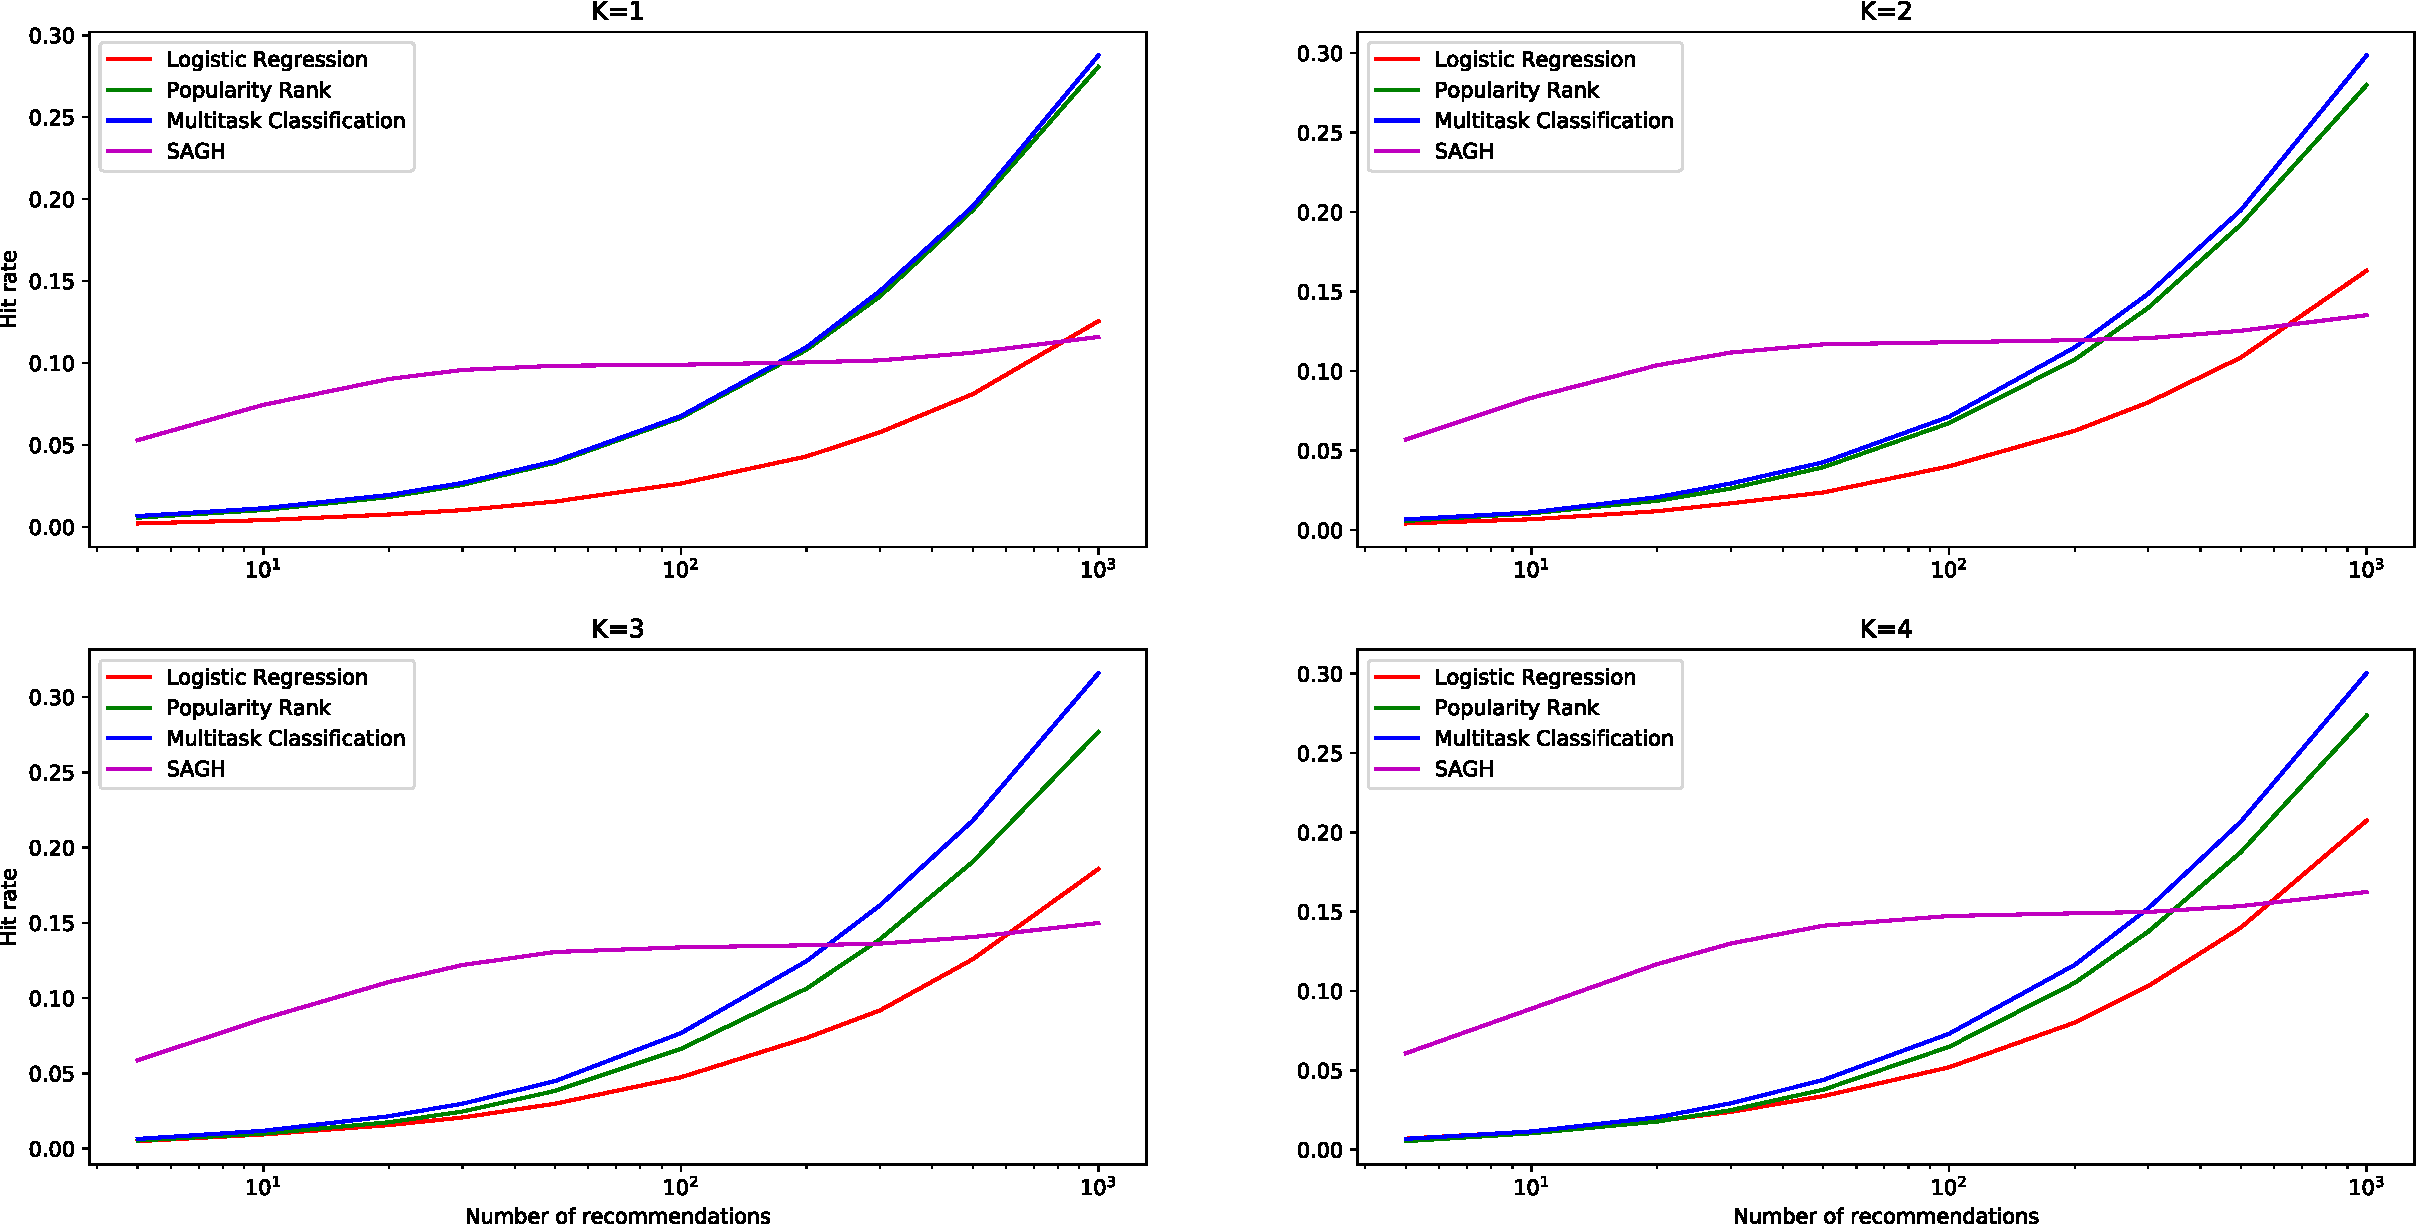
\includegraphics[width=\linewidth]{fig/30music-2.pdf}
\caption{Hit rates given $K=1,2,3,4$ seed songs on 30Music dataset.}
\end{figure*}


\subsection{New song recommendation}
\label{ssec:newsongrec}

We hold 5,000 and 10,000 of the latest released songs for test in the 30Music and AotM-2011 dataset, respectively.
For each song in test set, we predict whether it will be included in a given playlist.
As a remark, the set of users are the same for training and test, 
and playlists where every song is in test set are removed during training,
further, we test for playlists that has songs in both training and test set.
Table~\ref{tab:stats_newsongrec} summarises the statistics of the two dataset used for this task.

To tune hyper-parameters, we hold a subset of songs in training set as the validation set, 
which is constructed using the same approach as the test test.

\begin{table}[!h]
\centering
\caption{Statistics of dataset for new song recommendation}
\label{tab:stats_newsongrec}
%\resizebox{\linewidth}{!}{
\small
\begin{tabular}{l|rrr}
\toprule
Dataset   & \#Playlists & \#Songs (train) & \#Songs (test) \\
\midrule
30Music   & 8,215       & 40,468          & 5,000 \\
AotM-2011 & 19,504      & 104,428         & 10,000 \\
\bottomrule
\end{tabular}
%}
\end{table}

%\begin{table}[!h]
\centering
\caption{Empirical results (R-Precision $\times 10^3$)}
%\resizebox{\linewidth}{!}{
\small
\begin{tabular}{l|cccc}
\toprule
{}            & & & & BR \\
\midrule
AotM-2011     &  &  &  & 0.92 \\
30Music       &  &  &  & 7.24 \\
\bottomrule
\end{tabular}
%}
\end{table}


